\section{What incompleteness costs}
\label{sec:completeness}

\subsection{One tracer: the missing-host model does not add bias}
\label{sec:completeness:single}

The first question is whether the completion of \S\ref{sec:methods:completion}
works at all when it is handed the correct missing-host budget. Imposing an
isotropic flux limit on the matched single-tracer catalog takes the completeness
within the detection horizon from \AncCompleteC\% down to \AncMeighteenC\%, with
the surviving host count falling from \AncCompleteNHosts\ to
\AncMeighteenNHosts\ and the fraction of sky pixels containing no catalogued
host rising from \AncCompleteEmpty\% to \AncMeighteenEmpty\%
(Figure~\ref{fig:anchored}a, Table~\ref{tab:anchored}). Over that range the
recovered expansion rate stays within \AncMaxSigCtl$\sigma$ of the
complete-catalog control, the largest departure being
\AncMaxOffCtl~\kmsmpc\ (Figure~\ref{fig:anchored}b), and no likelihood
evaluation is inadmissible at any level. Replacing three-quarters of the
observed hosts inside the horizon by a modelled budget, and leaving nearly half
the sky without a catalogued host, adds no detectable bias to the distance scale.

The price is width. The 68\% interval grows by up to \AncMaxGrowth$\times$
(Figure~\ref{fig:anchored}c), which is what one expects when observed hosts are
replaced by a smooth prior, and it does not grow monotonically: the per-level
precision is a single realisation, with half-widths between \AncHwLo\ and
\AncHwHi~\kmsmpc, so the level-to-level ordering of the widths is not itself
meaningful.

Two limits on this statement. Every level, including the complete-catalog
control, sits low by roughly \AncCompleteOffAbs--\AncMtwentyOffAbs~\kmsmpc; that
pedestal is the offset of \S\ref{sec:budget} and not a completeness effect,
which is why the comparison here is differential. And with per-level precision
of order \AncHwLo--\AncHwHi~\kmsmpc, a bias smaller than about
\AncHwLo~\kmsmpc\ would not have been detected; the density model's own shape
residual, \AncResidHorizon\% within the horizon, sets a second floor of the same
character.

\begin{figure*}
\centering
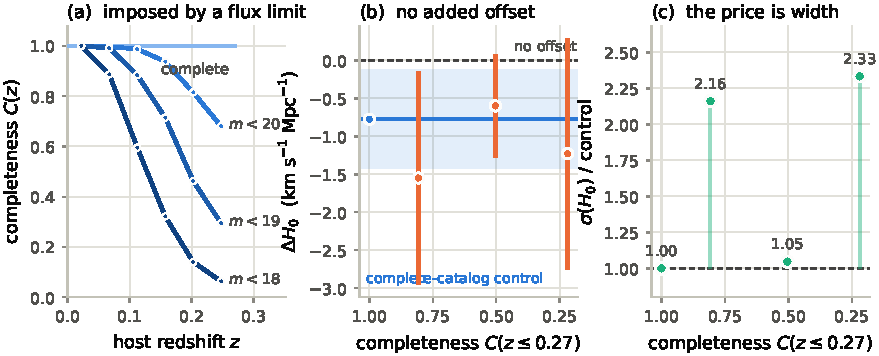
\includegraphics[width=\textwidth]{figures/fig_completeness_anchored.pdf}
\caption{Single-tracer flux-limit ladder with the tracer density anchored at the
truth. \emph{(a)} the completeness the flux limits impose across the detection
horizon, which declines with redshift as a flux-limited survey's does rather
than being cut off. \emph{(b)} the recovered expansion rate at each level; the
band is the complete-catalog control's own 68\% interval, and the largest
departure from it is \AncMaxSigCtl$\sigma$. \emph{(c)} the 68\% half-width as a
factor against that control. Error bars and the band are 68\% intervals from
single realisations, so the ordering of the widths between levels is not
significant; the range, up to \AncMaxGrowth$\times$, is.
\label{fig:anchored}}
\end{figure*}

\begin{deluxetable*}{lccccccc}
\tablecaption{Single-tracer flux-limit ladder. Completeness $C$ is quoted within the detection horizon $z\le\AncZref$. Offsets are relative to the true expansion rate; the last three columns are differential against the complete-catalog control. \label{tab:anchored}}
\tablehead{\colhead{level} & \colhead{hosts} & \colhead{$C$ (\%)} & \colhead{empty sky (\%)} & \colhead{$\Delta H_0$} & \colhead{vs.\ control} & \colhead{$\sigma$} & \colhead{width $\times$}}
\startdata
complete & 1\,000\,000 & 100.0 & 0.0 & $-0.78\pm0.65$ & $+0.00$ & 0.0 & 1.00 \\
$m<20$ & 20\,369 & 80.7 & 0.0 & $-1.55\pm1.41$ & $-0.77$ & 0.5 & 2.16 \\
$m<19$ & 7\,019 & 50.4 & 9.8 & $-0.60\pm0.68$ & $+0.18$ & 0.2 & 1.05 \\
$m<18$ & 2\,236 & 21.9 & 47.4 & $-1.23\pm1.52$ & $-0.45$ & 0.3 & 2.33 \\
\enddata
\end{deluxetable*}


\subsection{Two tracers: the fraction barely notices}
\label{sec:completeness:two}

The measurement that matters for survey design is what incompleteness does to
\fagn, and the answer is much less than what it does to \Hz. Putting the matched
two-tracer mock through the same flux-limit ladder --- the same events
throughout, only the catalogs thinned --- takes the completeness within the
range the events occupy from \IncCompleteC\ to \IncMeighteenC, the catalogued
AGN inside the horizon from \IncCompleteAgnInHorizon\ to
\IncMeighteenAgnInHorizon, and the fraction of sky with no catalogued AGN from
\IncCompleteAgnEmpty\% to \IncMeighteenAgnEmpty\%. Across that
\IncCRange-fold loss of sparse-tracer hosts, the joint 68\% half-width on the
fraction grows by \IncFacFMax$\times$ while that on the expansion rate grows by
\IncFacHzeroMax$\times$ (Figure~\ref{fig:twotracer}a,
Table~\ref{tab:twotracer}).

Three features of that ladder are worth stating plainly.

\emph{The first rungs are nearly free for the distance scale.} $\sigma(\Hz)$
grows by only \IncFacHzeroFirst$\times$ at the first rung and reaches
\IncFacHzeroMax$\times$ only at the faint end, non-monotonically in between;
as in \S\ref{sec:completeness:single} the per-level widths are single
realisations, so the rung-to-rung ordering is not itself meaningful, while
the overall range is. The reason the cost is so low is that the hosts a flux
limit removes first lie beyond the gravitational-wave horizon, where they
contribute prior weight at redshifts no event can occupy; only once the limit
starts removing hosts the events actually need does the width grow
appreciably. (On the mock as first generated this ladder showed an apparent
\IncPreFacHzeroGain\% \emph{improvement} at intermediate depth,
$\sigma(\Hz)$ falling to \IncPreFacHzeroMin$\times$ its complete-catalog
value. That gain does not survive the generator repair of
\S\ref{sec:budget:oracle}: it was a property of the defective posterior
construction interacting with this realisation, not of the survey --- a
concrete caution against reading structure into single-realisation width
ladders.)

\emph{The fraction's precision is nearly completeness-independent.} What
identifies \fagn\ is the contrast between the two completed tracer priors, and
the completion preserves that contrast: as observed hosts vanish, each tracer's
prior migrates onto its own smooth $n_{0,k}\,(\dd V_c/\dd z)(1+z)^{\delta_k}$
field, and the two fields still differ by the number-density ratio that carried
the signal to begin with. The informativeness of the \emph{design} is therefore
almost independent of how deep the survey is --- as long as $n_{0,k}$ is known,
which \S\ref{sec:density} shows is the whole of the caveat.

\emph{Every level stays evaluable.} Inadmissible cells fall from \IncRejMax\ to
\IncRejMin\ of \IncCompleteCells\ along the ladder and never approach the peak,
with a posterior mass adjacent to them of at most $\IncMassAdjMax$. The
selection integral's effective sample size \emph{rises}, from
$\IncCompleteNeff \times 10^3$ to $\IncMeighteenNeff \times 10^3$, because the
incomplete model's target is increasingly dominated by the smooth
out-of-catalog term, which the population branch of the proposal covers well.
This is the opposite of the failure mode of \S\ref{sec:selection}.

\subsection{Is that width real?}
\label{sec:completeness:null}

A width that is nearly flat across a sixfold change in completeness invites the
suspicion that it is set by something other than the data, so we measured what
the same analysis returns when the data cannot inform it. Permuting the
per-event sky positions among events preserves every sky patch, every distance
and every localisation area, and destroys only the pairing between an event's
distance and its own host's redshift. The permuted analysis returns a posterior
that is \emph{just as narrow} --- \IncCompleteNullRatio\ times the measured
width at the complete rung --- but centred at $\fagn = \IncCompleteNullMed$
instead of \IncCompleteFscan, a displacement of \IncCompleteSep\ measured widths
(Figure~\ref{fig:twotracer}b).

Read correctly this validates the measurement rather than undermining it. For a
mixture weight the likelihood's curvature is a property of how distinguishable
the two host priors are, which is a property of the survey design and not of the
realisation; a width that barely responds to the data is what that predicts.
What must be data-driven is the \emph{location}, and it is, by nearly five
widths. It also supplies the right degradation statistic for the AGN
identification itself, which combines width and displacement: the peak-to-null
separation falls from \IncCompleteSep\ widths at complete to \IncMeighteenSep\ at
$C = \IncMeighteenC$, a loss of \IncSepLoss\%
(Figure~\ref{fig:twotracer}c). That is close to the \IncFacFMax$\times$ width
figure and far from the \IncFacHzeroMax$\times$ one, so it is the fraction's
robustness and not the distance scale's that carries over.

\begin{figure*}
\centering
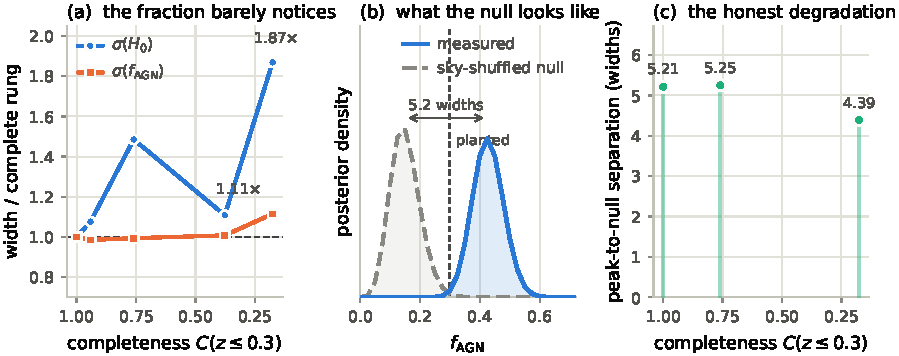
\includegraphics[width=\textwidth]{figures/fig_completeness_twotracer.pdf}
\caption{Two-tracer flux-limit ladder at fixed data, with both tracer densities
anchored at the truth. \emph{(a)} joint 68\% half-widths as factors against the
complete-catalog rung: the fraction degrades by \IncFacFMax$\times$ while the
expansion rate degrades by up to \IncFacHzeroMax$\times$, non-monotonically,
with the first rung costing only \IncFacHzeroFirst$\times$.
\emph{(b)} the measured fraction against its sky-shuffled null at the complete
rung; the null is equally narrow but sits \IncCompleteSep\ widths away.
\emph{(c)} that separation along the ladder, the degradation statistic for the
AGN identification itself.
\label{fig:twotracer}}
\end{figure*}

\begin{deluxetable*}{lcccccccccc}
\tablecaption{Two-tracer flux-limit ladder at fixed data. $C$ and the host count are for the sparse tracer within $z\le\IncZref$; $\sigma$ are 68\% half-widths from the joint $(H_0,f_{\rm AGN})$ grid, with the factor against the complete rung beside each. The last column is the separation between the measured $f_{\rm AGN}$ peak and its sky-shuffled null, in data widths. \label{tab:twotracer}}
\tablehead{\colhead{level} & \colhead{$C$} & \colhead{AGN in horizon} & \colhead{empty (\%)} & \colhead{$N_{\rm eff}/10^3$} & \colhead{$\sigma(H_0)$} & \colhead{$\times$} & \colhead{$\sigma(f_{\rm AGN})$} & \colhead{$\times$} & \colhead{separation}}
\startdata
complete & 1.000 & 154 & 37.5 & 147 & 0.767 & 1.00 & 0.0530 & 1.00 & 5.21 \\
$m<21$ & 0.942 & 145 & 94.5 & 166 & 0.826 & 1.08 & 0.0522 & 0.99 & \nodata \\
$m<20$ & 0.760 & 117 & 97.9 & 173 & 1.139 & 1.48 & 0.0527 & 0.99 & 5.25 \\
$m<19$ & 0.377 & 58 & 99.4 & 192 & 0.850 & 1.11 & 0.0534 & 1.01 & \nodata \\
$m<18$ & 0.175 & 27 & 99.8 & 221 & 1.433 & 1.87 & 0.0591 & 1.11 & 4.39 \\
\enddata
\end{deluxetable*}


\subsection{How to read the centres}
\label{sec:completeness:centres}

At every rung of the two-tracer ladder, including the complete one, the fraction
recovers high --- \IncCompleteF\ down to \IncMeighteenF\ against a planted
\IncFTruth\ --- so it is not a completeness effect. The expansion-rate
centres, by contrast, carry no common offset: they scatter from
\IncHzeroOffLo\ to \IncHzeroOffHi~\kmsmpc\ about the truth along the ladder,
consistent with the catalog-realisation term measured in \S\ref{sec:scatter}
(\SdsFixHzeroScatter~\kmsmpc\ of scatter per realisation) for a single shared
host field. (Before the generator repair the ladder sat uniformly low, with offsets from
\IncPreHzeroOffLo\ to \IncPreHzeroOffHi~\kmsmpc; the repair removed the
common offset and left the realisation scatter.) The high
fraction is a change of \emph{estimator} rather than of data: the same mock and
the same events under the complete-catalog limit give $\fagn = \DeepFixFTgtMed$
(\S\ref{sec:selection}), and switching to the completed model with the true
per-tracer anchor gives \IncCompleteFscan, \IncCompleteFscanSig$\sigma$ high
at the complete rung. The mechanism is specific and worth
spelling out, because it is generic to sparse tracers. The completion cannot
distinguish ``no AGN here'' from ``no AGN observed here'', and with only
\IncCompleteAgnInHorizon\ catalogued AGN inside the horizon the Poisson noise in
$\dd N_{\rm obs}/\dd z$ is large enough that Equation~(\ref{eq:completeness})
returns $C_{\rm AGN}(z) < 1$ in many bins even when the catalog is genuinely
complete. A missing-AGN budget is then manufactured out of shot noise and
deposited in empty pixels, where it lets events be AGN-hosted. This is the
sparse-tracer form of the degeneracy between the mixture weight and the tracer
density, and it is what \S\ref{sec:density} measures.
